\section{Maximal operators along separated directions in $\R^{2}$}
Kakeya maximal operators on $\R^{2}$ were was first estimated in \cite{MR0447949} (for a nice proof of a stronger result see \cite{MR2550196}).
Kakeya maximal operators are controlled by maximal operators along separated directions, and these were first estimated in \cite{MR0438022}.
In this section we prove the sharp estimate for such operators obtained in \cite{MR0481883}.

\begin{lemma}
\label{lem:Stromberg-covering}
Let $N\geq 2$ be an integer, $\Omega$ a $1/N$-separated set of directions in $\R^{2}$ and let $\calR$ a set of rectangles in $\R^{2}$ for which one of the sides points in a direction in $\Omega$.
Then there exists a subset $\calG \subset \calR$ such that
\begin{align}
\label{eq:int-sum^2}
\int_{\R^{2}} \left(\sum_{R \in \calG} \one_{R}(x)\right)^{2} \dif x
&\leq C \abs[\big]{ \bigcup_{R\in\calG} R }, \\
\label{eq:cover}
\abs[\big]{ \bigcup_{R \in \calR} R }
&\leq C (\log N) \abs[\big]{ \bigcup_{R \in \cal G} R }.
\end{align}
\end{lemma}
The separation hypothesis on $\Omega$ implies that $\abs{\Omega} \lesssim N$.
The separation hypothesis was replaced by this cardinality hypothesis in \cite{MR1681088} (an alternative proof appeared in \cite{MR1979927}).
We will only use separated $\Omega$'s.
\begin{proof}
Without loss of generality we may assume that $\calR$ is finite.
Partitioning $\calR$ into boundedly many pieces and using rotation invariance we may assume that the long sides of rectangles in $\calR$ point in the directions in $\Omega$ and that these directions are all within $1/10$ of some fixed direction.

We choose $\calG = \Set{ R_{1}, R_{2}, \dotsc }$ in the following way.
Suppose that $R_{1},\dotsc,R_{n-1}$ are already chosen.
Then let $R_{n}$ be a rectangle in $\calR$ with the longest long side subject to the condition
\begin{equation}
\label{eq:rect-choice}
\sum_{j=1}^{n-1} \abs{ R_{j} \cap R_{n} }
\leq
\frac{1}{2} \abs{ R_{n} }
\end{equation}
if such $R_{n}$ exists, or stop the construction otherwise.
By \eqref{eq:rect-choice} we have
\[
\abs[\big]{ R_{n} \setminus \cup_{j<n} R_{j} }
\geq
\abs{ R_{n} } - \sum_{j=1}^{n-1} \abs{ R_{j} \cap R_{n} }
\geq
\frac{1}{2} \abs{ R_{n} },
\]
and it follows that
\begin{multline}
\int_{\R^{2}} \left( \sum_{n} \one_{R_{n}} \right)^{2}
\leq
2 \sum_{j \leq n} \abs{ R_{j} \cap R_{n} }
\leq
3 \sum_{n} \abs{ R_{n} }\\
\leq
6 \sum_{n} \abs[\big]{ R_{n} \setminus \cup_{j<n} R_{j} }
=
6 \abs[\big]{ \cup_{n} R_{n} }.
\end{multline}
This shows \eqref{eq:int-sum^2}.
By the weak type $(1,1)$ inequality for the Hardy--Littlewood maximal operator $M$ the remaining inequality \eqref{eq:cover} will follow from
\begin{equation}
\cup_{R \in \calR \setminus \calG} R
\subset \Set{ M \bigl( \sum_{n} \one_{\tilde{R}_{n}} \bigr) > c / \log N},
\end{equation}
where $\tilde{R}_{n}$ is the rectangle with the same center, width, and orientation as $R_{n}$, and length multiplied by $4$.

If $R \in \calR\setminus\calG$, then \eqref{eq:rect-choice} fails for $R$ for all large $n$.
Let $n$ be the smallest index for which \eqref{eq:rect-choice} fails.
Then
\[
\sum_{j=1}^{n-1} \abs{ R_{j} \cap R }
\geq
\frac{1}{2} \abs{ R }
\]
and the long side of $R_{j}$ is longer than the long side of $R$ for all $j < n$, since otherwise $R_{j}$ could not have been selected.
Denote by $\theta_{j}$ the angle between long sides of $R$ and $R_{j}$ and by $w_{j}$ the width of $R_{j}$.

\begin{figure*}
\begin{center}
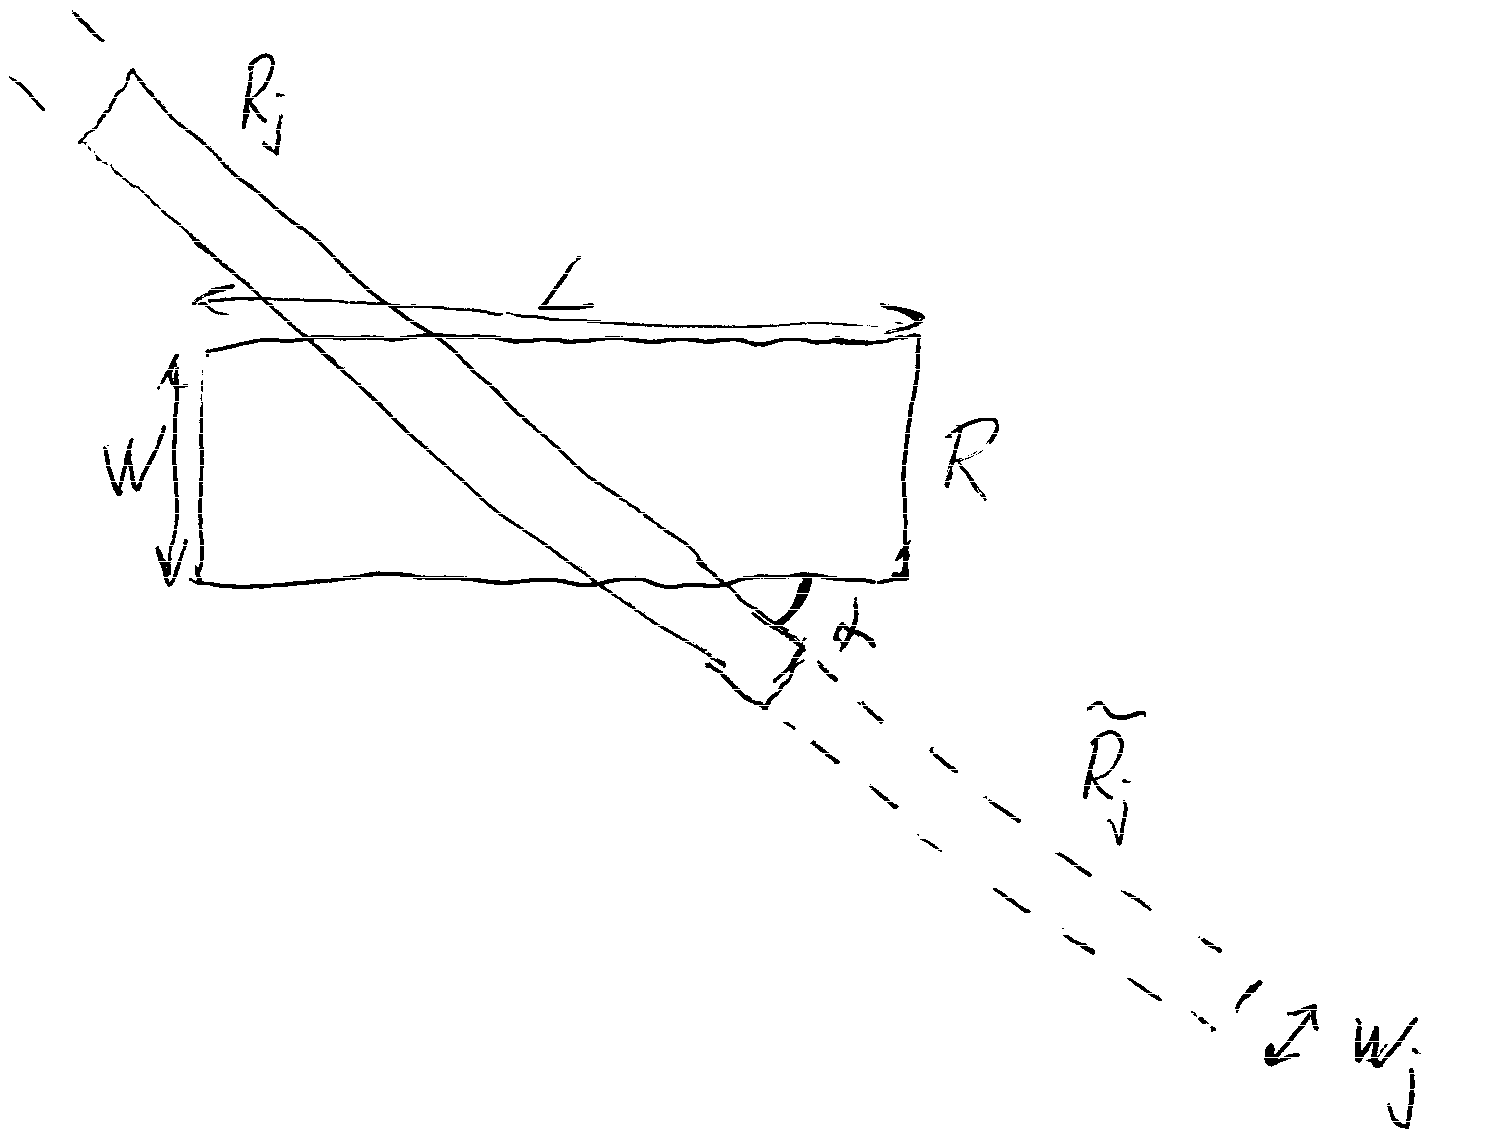
\includegraphics[height=5cm]{Stromberg-covering.png}
\end{center}
\end{figure*}

Let $L$ be the length of $R$, $W$ its width, and $0 \leq \alpha \leq 1/10$.
Let $s := 8 \max ( W, \alpha L )$.
Suppose that $\alpha \leq \theta_{j} \leq 2 \alpha$.
We claim that for every cube $Q$ with side length $s$ and center in $R$ we have
\[
\frac{ \abs{\tilde{R}_{j} \cap Q} }{ \abs{Q} }
\gtrsim
\frac{ \abs{R_{j} \cap R} }{ \abs{R} }.
\]
If $w_{j} \geq s$, then in fact both sides are $\sim 1$, so assume $w_{j} < s$.
Then
\[
\abs{\tilde{R}_{j} \cap Q} \gtrsim s w_{j},
\]
and also
\[
\abs{ R_{j} \cap R } \lesssim \min( Lw_{j}, Ww_{j}/\alpha ).
\]
Hence
\[
\frac{ \abs{R_{j} \cap R} }{ \abs{R} }
\lesssim
w_{j} \min( L, W/\alpha ) / (LW)\\
=
w_{j} / \max( W, \alpha L )
\sim
w_{j} / s
\lesssim
\frac{ \abs{\tilde{R}_{j} \cap Q} }{ \abs{Q} }
\]
as claimed.

By the pigeon principle there exists $\alpha \in \Set{ 0, 2^{0} \frac{2\pi}{N}, 2^{1}\frac{2\pi}{N}, \dotsc }$ such that for the set $J = \Set{ j<n \given \alpha \leq \theta_{j} \leq 2 \alpha }$ we have
\[
\sum_{j \in J} \abs{ R_{j} \cap R }
\gtrsim
(\log N)^{-1} \abs{ R }.
\]
Considering the cube $Q$ with side length $s$ centered at any $x \in R$ we obtain
\begin{align*}
M \bigl( \sum_{n} \one_{\tilde{R}_{n}} \bigr) (x)
&\geq
M \bigl( \sum_{j\in J} \one_{\tilde{R}_{j}} \bigr) (x)\\
&\geq
\abs{Q}^{-1} \sum_{j\in J} \abs{\tilde{R}_{j} \cap Q}\\
&\geq
\sum_{j\in J} \abs{R}^{-1} \abs{R_{j} \cap R}\\
&\gtrsim
(\log N)^{-1}.
\qedhere
\end{align*}
\end{proof}

\begin{theorem}[{\cite{MR0481883}}]
\label{thm:Stromberg-weak-2,2}
Let $N\geq 2$ be an integer and $\Omega$ a $1/N$-separated set of directions in $\R^{2}$.
Let $M_{\Omega}$ be the maximal operator associated to averaing over rectangles one of whose sides points in a direction in $\Omega$.
Then
\begin{equation}
\label{eq:Stromberg-weak-2,2}
\norm{ M_{\Omega} f }_{2,\infty} \lesssim (\log N)^{1/2} \norm{ f }_{2}.
\end{equation}
\end{theorem}
\begin{proof}
Let $\calR$ be the set of all rectangles $R$ with sides pointing in directions in $\Omega$ for which $\abs{R}^{-1} \int_{R} \abs{f} > \lambda$.
Let $\calG \subset \calR$ be as in Lemma~\ref{lem:Stromberg-covering}.
Then
\[
\lambda^{2} \abs[\big]{ \bigcup_{R \in \calG} R }^{2}
\leq
\lambda^{2} \Bigl( \sum_{R} \abs{R} \Bigr)^{2}
<
\Bigl( \sum_{R} \int_{R} \abs{f} \Bigr)^{2}
\leq
\norm{f}_{2}^{2} \norm{ \sum_{R\in\calG} \one_{R} }_{2}^{2}
\lesssim
\norm{f}_{2}^{2} \abs[\big]{ \bigcup_{R \in \calG} R },
\]
and it follows that
\[
\abs{ \Set{ M_{\Omega} f > \lambda } }
=
\abs[\big]{ \bigcup_{R \in \calR} R }
\lesssim
(\log N)
\abs[\big]{ \bigcup_{R \in \calG} R }
\lesssim
(\log N) \lambda^{-2} \norm{f}_{2}^{2}.
\qedhere
\]
\end{proof}

We will need the following interpolation argument.
It was already used in \cite{MR0481883}, but the proof was not written down, so several later papers prove versions of this result \cite{MR1261427,MR1681088,MR2680067}.
\begin{lemma}
\label{lem:3-point-weak-type-interpolation}
Let $N\geq 2$, $1\leq p < 2$, and $T$ be a quasisubadditive operator such that
\[
\norm{Tf}_{p,\infty} \leq N \norm{f}_{p},
\quad
\norm{Tf}_{\infty} \leq N \norm{f}_{\infty},
\quad
\norm{Tf}_{2,\infty} \leq \norm{f}_{2}.
\]
Then
\[
\norm{Tf}_{2} \lesssim (\log N)^{1/2} \norm{f}_{2}.
\]
\end{lemma}
\begin{proof}
The basic idea is to use the layer cake representation
\[
\norm{Tf}_{2}^{2} \sim \int_{0}^{\infty} \lambda \abs{ \Set{ Tf > \lambda } } \dif \lambda,
\]
for each $\lambda$ decompose
\[
f = f \one_{\abs{f} < N^{\alpha}\lambda} + f \one_{ N^{\alpha}\lambda \leq \abs{f} \leq N^{\beta}\lambda} + f \one_{N^{\beta}\lambda < \abs{f}},
\]
use the three different estimates for these pieces and optimize $\alpha,\beta$.
The rest is an exercise.
\end{proof}

The various versions of Lemma~\ref{lem:3-point-weak-type-interpolation} in \cite{MR1261427,MR1681088,MR2680067} have a common formulation in terms of real interpolation spaces.
We record it here using notation and results from \cite{MR0482275}.
This general version will not be used in this course.
\begin{lemma}
\label{lem:3-point-real-interpolation}
Let $\bar{A}, \bar{B}$ be compatible couples of Banach spaces, $0 < \theta < 1$, and $1\leq s \leq q \leq \infty$.
Let $N\geq 2$ and let $T$ be a (quasisub-)additive operator such that
\[
\norm{Ta}_{B_{0}} \leq N \norm{a}_{A_{0}},
\quad
\norm{Ta}_{B_{1}} \leq N \norm{a}_{A_{1}},
\quad
\norm{Ta}_{B_{\theta,\infty}} \leq \norm{a}_{A_{\theta,s}}.
\]
Then
\begin{equation}
\label{eq:3-point-real-interpolation}
\norm{Ta}_{B_{\theta,q}} \lesssim (\log N)^{1/s} \norm{a}_{A_{\theta,q}}.
\end{equation}
\end{lemma}
Interpolating between \eqref{eq:3-point-real-interpolation} with $q=\infty$ and the $A_{\theta,s} \to B_{\theta,\infty}$ estimate in the hypothesis using the reiteration theorem we further obtain
\begin{equation}
\label{eq:3-point-real-interpolation:r->infty}
\norm{Ta}_{B_{\theta,\infty}} \lesssim (\log N)^{1/s-1/r} \norm{a}_{A_{\theta,r}},
\quad
s \leq r \leq \infty.
\end{equation}
This allows to recover \cite[Proposition 5(i)]{MR1261427}.
\begin{proof}
By the fundamental lemma of interpolation theory there exists a decomposition
\[
a = \sum_{j\in\Z} a_{j}
\quad
\text{ with }
J(2^{j},a_{j}) \lesssim K(2^{j},a).
\]
By subadditivity of the $K$-functional we split
\[
K(2^{j}, Ta)
\lesssim
K(2^{j}, T (\sum_{k<-A} a_{j+k}) )
+
K(2^{j}, T (\sum_{\abs{k} \leq A} a_{j+k}) )
+
K(2^{j}, T (\sum_{k > A} a_{j+k}) ).
\]
Now we estimate the individual terms.
\begin{multline*}
K(2^{j}, T (\sum_{k<-A} a_{j+k}) )
\leq
\norm{ T (\sum_{k<-A} a_{j+k}) }_{B_{0}}
\leq
N \norm{ \sum_{k<-A} a_{j+k} }_{A_{0}}\\
\leq
N \sum_{k<-A} \norm{ a_{j+k} }_{A_{0}}
\leq
N \sum_{k<-A} J(2^{j+k}, a_{j+k} )
\leq
N \sum_{k<-A} K(2^{j+k}, a )
\end{multline*}
\begin{multline*}
K(2^{j}, T (\sum_{\abs{k} \leq A} a_{j+k}) )
\leq
2^{j\theta} \norm{ T (\sum_{\abs{k} \leq A} a_{j+k}) }_{B_{\theta,\infty}}
\leq
2^{j\theta} \norm{ \sum_{\abs{k} \leq A} a_{j+k} }_{A_{\theta,s}}\\
\lesssim
2^{j\theta} \Bigl( \sum_{\abs{k} \leq A} (2^{-(j+k)\theta} J(2^{j+k}, a_{j+k}) )^{s} \Bigr)^{1/s}
\lesssim
2^{j\theta} \Bigl( \sum_{\abs{k} \leq A} (2^{-(j+k)\theta} K(2^{j+k}, a) )^{s} \Bigr)^{1/s}.
\end{multline*}
\begin{multline*}
K(2^{j}, T (\sum_{k>A} a_{j+k}) )
\leq
2^{j} \norm{ T (\sum_{k>A} a_{j+k}) }_{B_{1}}
\leq
2^{j} N \norm{ \sum_{k>A} a_{j+k} }_{A_{1}}\\
\leq
2^{j} N \sum_{k>A} \norm{ a_{j+k} }_{A_{1}}
\leq
2^{j} N \sum_{k>A} 2^{-(j+k)} J(2^{j+k}, a_{j+k} )
\leq
N \sum_{k>A} 2^{-k} K(2^{j+k}, a ).
\end{multline*}
\begin{multline*}
\norm{Ta}_{B_{\theta,q}}
\sim
\Bigl( \sum_{j\in\Z} (2^{-j\theta} K(2^{j}, Ta) )^{q} \Bigr)^{1/q}\\
\lesssim
\Bigl( \sum_{j\in\Z} \Bigl( \sum_{k<-A} 2^{k\theta} N 2^{-(j+k)\theta} K(2^{j+k}, a)
+ \bigl( \sum_{\abs{k} \leq A} (2^{-(j+k)\theta} K(2^{j+k}, a) )^{s} \bigr)^{1/s}\\
+ \sum_{k>A} 2^{-k(1-\theta)} N 2^{-(j+k)\theta} K(2^{j+k}, a) \Bigr)^{q} \Bigr)^{1/q}\\
\leq
\sum_{k<-A} 2^{k\theta} N \Bigl( \sum_{j\in\Z} \Bigl( 2^{-(j+k)\theta} K(2^{j+k}, a) \Bigr)^{q} \Bigr)^{1/q}\\
+ \Bigl( \sum_{j\in\Z} \Bigl( \bigl( \sum_{\abs{k} \leq A} (2^{-(j+k)\theta} K(2^{j+k}, a) )^{s} \bigr)^{1/s} \Bigr)^{q} \Bigr)^{1/q}\\
+ \sum_{k>A} 2^{-k(1-\theta)} N \Bigl( \sum_{j\in\Z} \Bigl( 2^{-(j+k)\theta} K(2^{j+k}, a) \Bigr)^{q} \Bigr)^{1/q}\\
\lesssim
\sum_{k<-A} 2^{k\theta} N \norm{a}_{A_{\theta,q}}
+ (2A+1)^{1/s} \norm{a}_{A_{\theta,q}}
+ \sum_{k>A} 2^{-k(1-\theta)} N \norm{a}_{A_{\theta,q}}.
\end{multline*}
Choosing $A \sim \log N$ we obtain the claim.
\end{proof}

\begin{corollary}
\label{cor:Stromberg-strong-2,2}
In the setting of Theorem~\ref{thm:Stromberg-weak-2,2} we have
\[
\norm{ M_{\Omega} f }_{2} \lesssim (\log N) \norm{ f }_{2}.
\]
\end{corollary}
\begin{proof}
Apply Lemma~\ref{lem:3-point-real-interpolation} to the operator $(\log N)^{-1} M_{\Omega}$ with estimate $O(N)$ for the $L^{p}\to L^{p}$ norm, $1<p<2$, estimate $O(1)$ for the $L^{\infty} \to L^{\infty}$ norm, and estimate \eqref{eq:Stromberg-weak-2,2} for the $L^{2} \to L^{2,\infty}$ norm.
\end{proof}

%%% Local Variables:
%%% mode: latex
%%% TeX-master: decoupling-notes
%%% End:
